
\section{What happens when a discriminatively pretrained network is finetuned?}
\label{sec:fine}
%Finetuning a network is the process of slowly updating pre-learned parameters to minimize a target loss function for a new task at hand. Since, CNNs consist of large number of parameters they are prone to overfitting when trained on small datasets. Finetuning can be considered as a method of transfer learning and recent results from \cite{Rcnn, Decaf} presented a strong case for this methodology boosting performance. Although, unsupervised pretraining has been widely studied in the multilayer network literature \cite{AmitGeman, DeepPre}, there is no work analysing the effect of fine-tuning on different layers of a discriminatively trained multilayer convolutional networks.

%We start our analysis by investigating how the discriminative capacity of different layers of the network changes as a result of finetuning. We measure discriminative capacity using the entropy of each layer  
%We start our analysis by investigating how the entropy of filters across different layers changes as a result of discriminative fine-tuning (see sec \ref{sub:fine-entropy}). Since, entropy of a filter can be evaluated at different threshold level of activations we propose the metric of Area under the Entropy curve (AuE) to judge changes in filter selectivity. Our main finding is that most of the learning during finetuning happens only in the top two fully connected layers. Motivated by this observation, we finetune networks for PASCAL detection and SUN-397 scene classification task by setting non-zero learning rates only in the top 2 layers (see sec\ref{sub:fine-fc-only}). We find this results in a negligible drop in performance and allows for moderate speed-ups in finetuning time. Other conclusions are presented in the sec \ref{sub:fine-discussion}.

Results from \cite{Rcnn} suggested that fine-tuning a discriminatively pre-trained network is a powerful method for task specific feature learning. Consequently, we studied the effect of fine-tuning on performance under the experimental setups of SUN-CLS and PASCAL-DET (section \ref{sub:effect-finetune}). We provide objective evidence that with less data, pre-training followed by fine-tuning is required for good performance, whereas with enough data, a CNN can be trained from scratch. We also find that fine-tuning with more data leads to better performance and this is used to establish the new state of art results on PASCAL-DET.

Given these results, it is important to understand the effect, fine-tuning has on the parameters of the CNN. Towards this end, we investigate the effect of fine-tuning for PASCAL-DET has on the discriminative capacity of individual features extracted from different layers of the CNN (section .) We find that discriminative capacity of individual features from layers 1 to 5 does not changes much, whereas features in layers 6 to 7 become substantially more discriminative. We use this observation to show that fine-tuning only the top two layers (i.e. 6,7) leads to similar performance as achieved by fine-tuning all layers on datasets of size PASCAL-DET and SUN-CLS. However, we also note that given larger datasets, fine-tuning only layers 6,7 is insufficient. This suggests that work such as (\todo{REF}) can benefit from fine-tuning all layers.        

\subsection{Effect of fine-tuning on performance}
\label{sub:effect-finetune}
\setlength{\tabcolsep}{2pt}
\begin{table}[t!]
\begin{center}
\caption{Comparing the performance of a CNN trained from scratch, pre-trained on Imagenet and fine-tuned for the particular task. VOC 2007 + 2012 data was used for training from scratch and fine-tuning for PASCAL-DET-2. }
\label{table:fine-effect}
\scalebox{0.9}{
\begin{tabular}{|l|ccc|ccc|ccc|}
\hline
Layer &  \multicolumn{3}{c|}{SUN-CLS} & \multicolumn{3}{c|}{PASCAL-DET} & \multicolumn{3}{c|}{PASCAL-DET-2} \\
\hline
  &    scratch & pre-train & fine-tune  & scratch & pre-train & fine-tune & scratch & pre-train & fine-tune\\
\hline
fc-7 & $40.2 \pm $ & $53.1 \pm 0.2$ & $56.8 \pm 0.2$ & 40.7 & 45.5 & 54.1 & 52.3 & 45.5 & 59.2 \\ 
\hline
\end{tabular}}
\end{center}
\end{table}
\setlength{\tabcolsep}{1.4pt}


\subsection{Effect of fine-tuning on network parameters}
\label{sub:fine-entropy}
The discriminative capacity of an individual filter is measured using the following procedure: Each image, when passed through the CNN produces a $p \times p$ heat-map of filter responses (e.g. p = 6, for conv-5 filter). This heat-map is vectorized (i.e. x(:) in matlab) into a vector of scores of length $p^2$. With each element of this vector we associate the class label of the image. Thus, for every image we have a score vector and a label vector of length $p^2$ each. Next, score and label vectors from N images are concatenated into a giant score and giant label vectors respectively of size $Np^2$ each. For a given score threshold, the entropy of the set of labels which have an associated score $\geq$ to this threshold is the class entropy of the filter. As this threshold changes, entropy traces out a curve which we call as the entropy curve. The Area under the Entropy curve (AuE), accounts for entropy at different thresholds and is used as a measure of discriminative capacity of the filter. Lower the value of AuE, the more discriminative is the filter. 

For characterizing the distribution of discriminative ability of all filters of a layer - filters were sorted according to their AuE. Then, the cumulative sum of this sorted list of AuE was calculated (called as Cumulative Area under Entropy (CAuE)). The $i^{th}$ entry of the CAuE list is the sum of entropies of the top $i$ most discriminative filters. The difference in the value of the $i^{th}$ entry before and after fine-tuning measures the changes in the individual entropy of the top $i$ most discriminative filters due to fine-tuning. For comparing results across different layers, the CAuE values are normalized to account for different number of filters in each layer. Specifically, the $i^{th}$ entry of the CAuE list is divided by $i$. This normalized CAuE is called the Mean Cumulative Area Under the Entropy Curve (MCAuE). A lower value of MCAuE indicates that the filters are more discriminative.

In order to summarize the class selectivity for a \emph{set} of filters, we sort them from the most selective to least selective and plot the average selectivity of the first $k$ filters while sweeping $k$ down the sorted list.
Figure \ref{fig:fine-entropy} shows the class selectivity for the sets of filters in layers 1 to 7 before and after fine-tuning (on VOC 2007 trainval).
Selectivity is measured using the ground truth boxes from PASCAL-DET-GT instead of a whole-image classification task to ensure that filter responses are a direct result of the presence of object categories of interest and not correlations with image background.

\begin{comment}
\begin{figure}[t!]
\centering
\subfloat{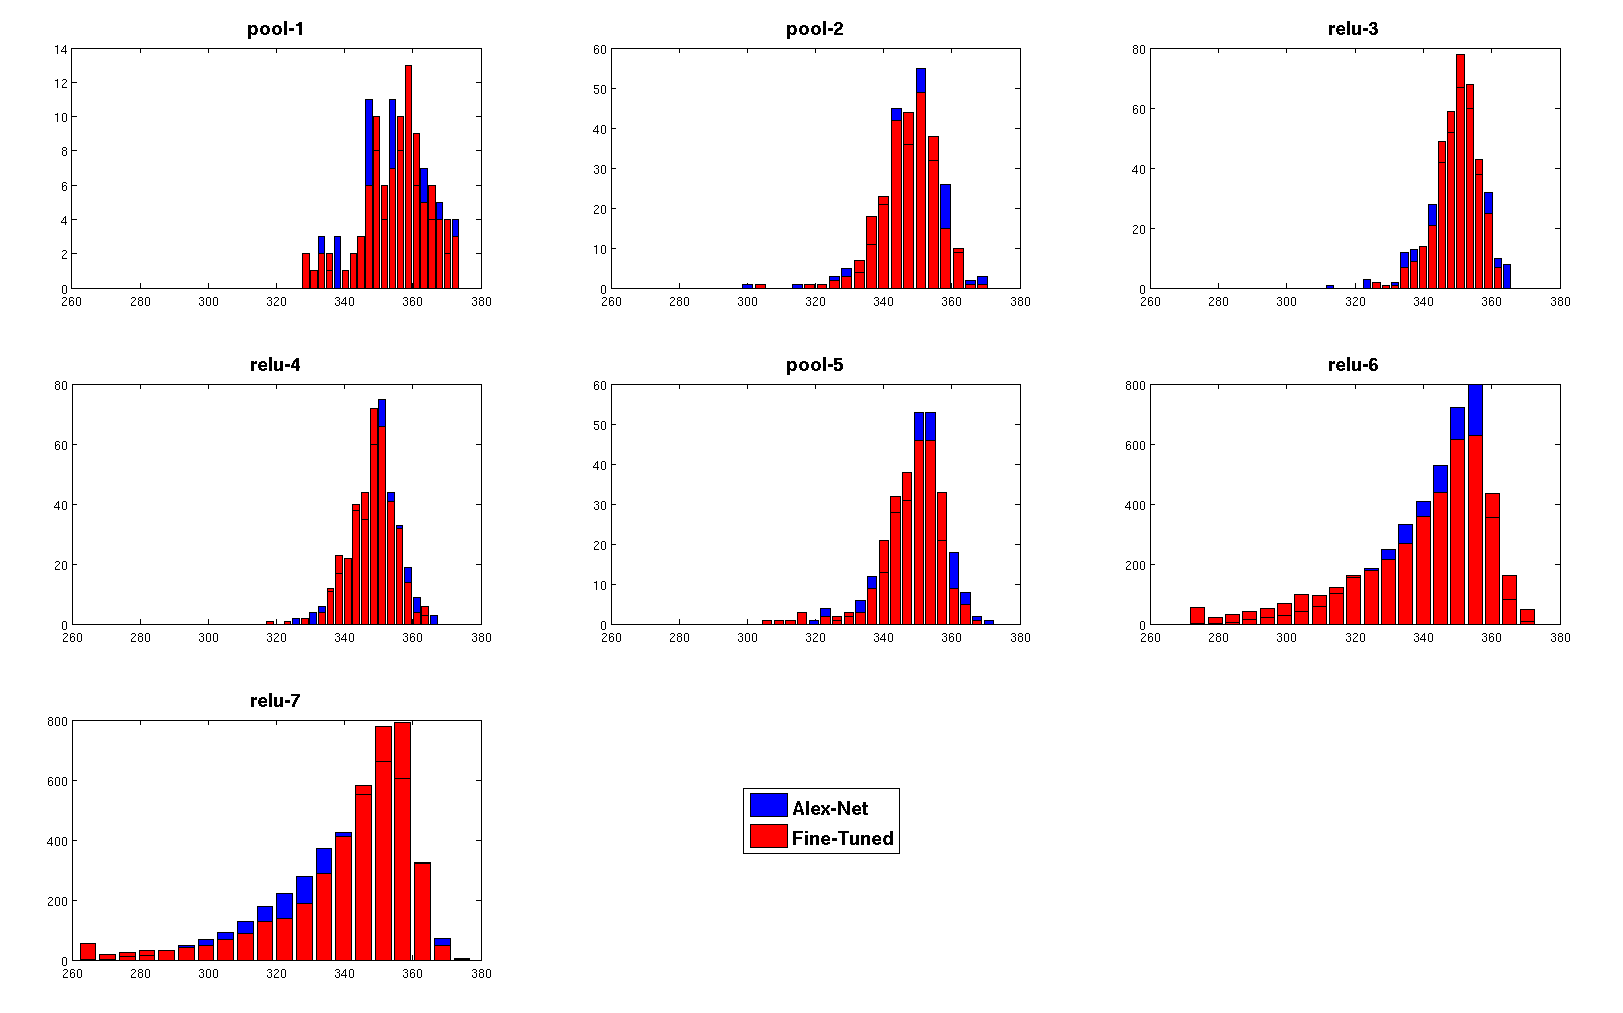
\includegraphics[height=6.5cm]{images/ent_hist.png}}
\caption{Distribution of AuE for different layers in Alex-Net and FT-Net. X-axis is the entropy and the Y-axis is the number of filters. Notice that the left tail for fc-6 and fc-7 becomes heavier after finetuning. This indicates that finetuning makes these filters more discriminative.}
\label{fig:fine-hist}
\end{figure}
\end{comment}

\begin{figure}[t!]
\centering
\subfloat{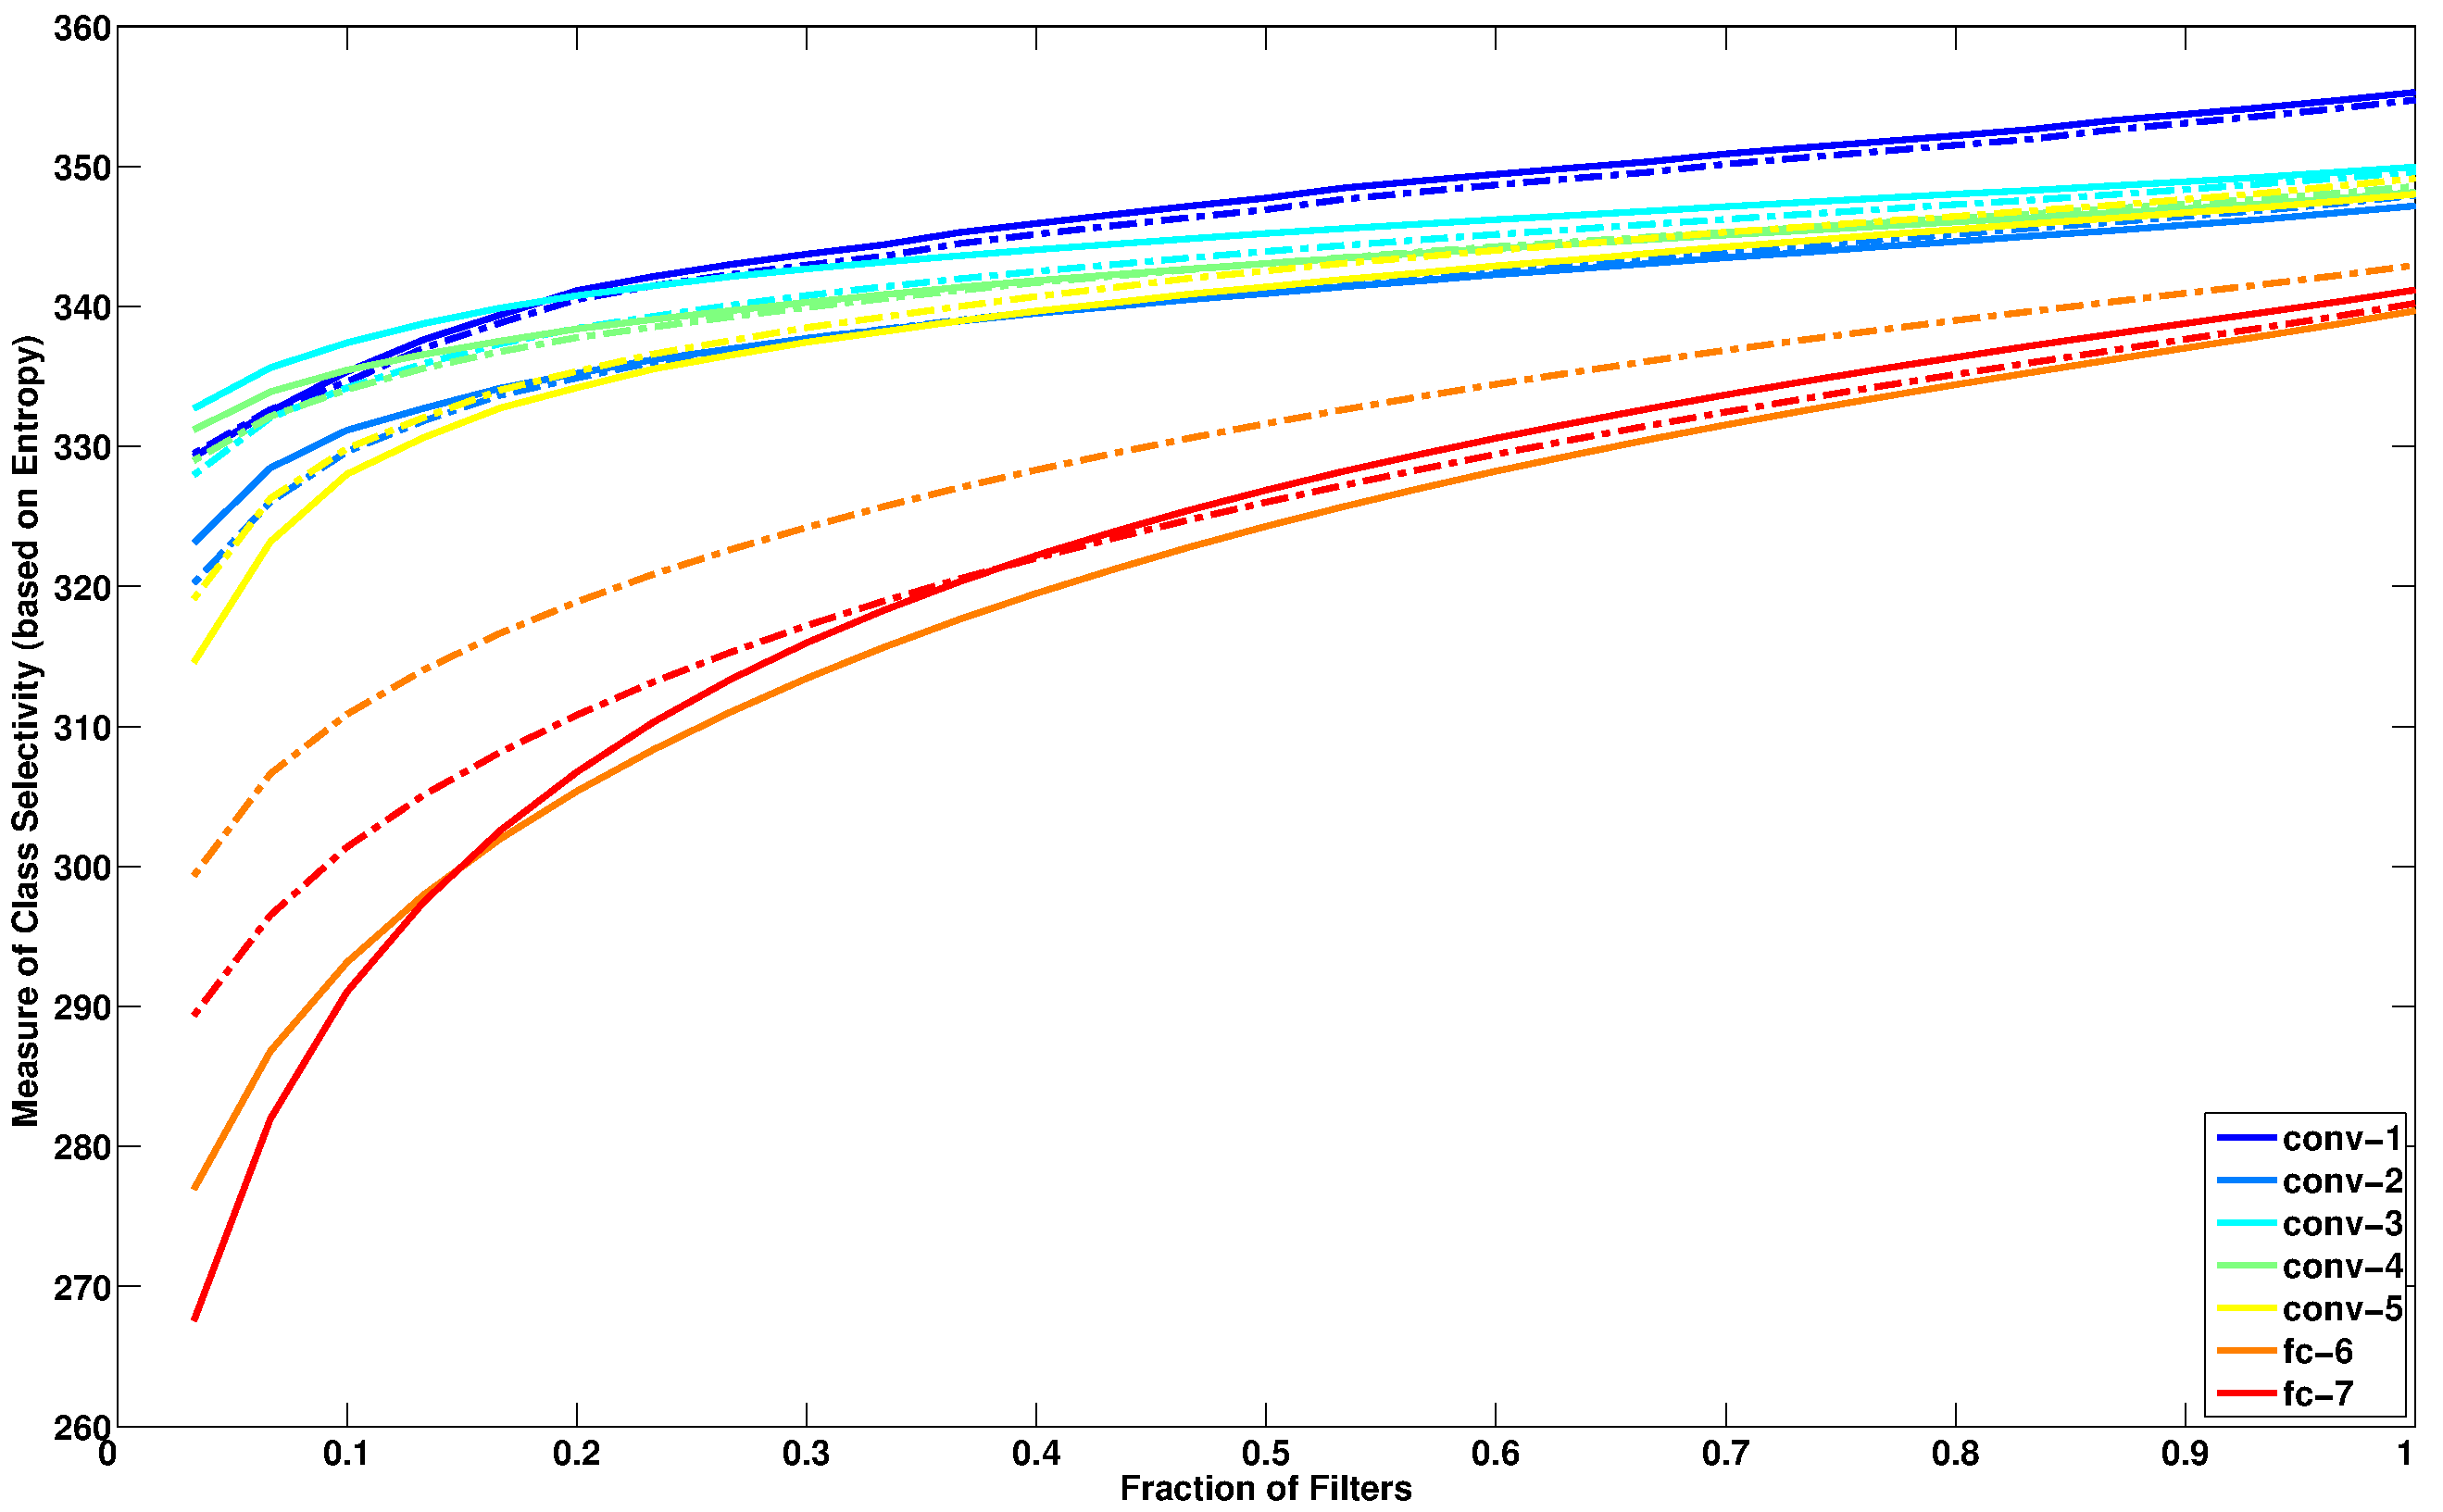
\includegraphics[scale=0.20]{images/MCAUE.pdf}}
\caption{The value of MCAuE (see text for definition) plotted against the fraction of filters (see sec \ref{sub:fine-entropy}) for all layers of Alex-Net (Dash-Dot line) and a fine-tuned network (Solid line). A lower value of MCAuE indicates that the layer is more discriminative. Although layers become more discriminative as we go higher up in the network (i.e. from layer 1 to 7), fine-tuning only seems to significantly effect the last two layers.}
\label{fig:fine-entropy}
\end{figure}

Figure \ref{fig:fine-entropy} shows that class selectivity increases from layer 1 to 7 for both networks.
This result is consistent with performance numbers reported in Table \ref{table:det-traj-classify}. 
However, it is interesting to note that entropy changes due to fine-tuning are only significant for layers 6 and 7. 
This observation indicates that fine-tuning only layers 6 and 7 may suffice for achieving good performance when fine-tuning data is limited. 
We test this hypothesis on SUN-CLS and PASCAL-DET by comparing the performance of a fine-tuned network (ft) with a network which is fine-tuned by only updating weights of fc-6 and fc-7 (fc-ft network). 
Results are summarized in Table \ref{table:fine-fc-ft}.
With small amounts of data, fine-tuning amounts to ``rewiring'' the fully connected layers.
However, when more fine-tuning data is available (PASCAL-DET+DATA), there is still substantial benefit from fine-tuning all network parameters.

\setlength{\tabcolsep}{2pt}
\begin{table}[t!]
\begin{center}
\caption{Comparison in performance on of Alex-Net, Finetuned Network(ft-net) and a network with only fc layers finetuned (fc-ft).}
\label{table:fine-effect}
\scalebox{0.9}{
\begin{tabular}{|l|cc|cc|cc|}
\hline
Layer &  \multicolumn{2}{c|}{SUN-CLS} & \multicolumn{2}{c|}{PASCAL-DET} & \multicolumn{2}{c|}{PASCAL-DET-2} \\
\hline
  &    ft & fc-ft  & ft & fc-ft & ft & fc-ft \\
\hline
fc-7 & $56.8 \pm 0.2$ & $56.2 \pm 0.1$ & 54.1 & 53.3 & 59.2 & 56.0 \\ 
\hline
\end{tabular}}
\end{center}
\end{table}
\setlength{\tabcolsep}{1.4pt}

We find that the final performance in the detection setup only drops by 0.8 points and by 0.6 points for scene-classification.  

\setlength{\tabcolsep}{1pt}
\begin{table}[t!]
\begin{center}
\caption{\todo{Include layer-wise results for PASCAL-DET-2?} for Evaluation of effect finetuning towards the task of object detection. (l5, l6, l7: layers 5, 6 and 7 of Alex Net)}
\label{table:det-fine}
\scalebox{0.75}{
\begin{tabular}{l|cccccccccccccccccccc||c}
\hline\noalign{\smallskip}
layer & aero & bike & bird & boat & bottle & bus & car & cat & chair & cow & table & dog & horse & mbike & person & plant & sheep & sofa & train & tv & mAP \\
\noalign{\smallskip}
\hline
l5 & 51.9 & 61.1 & 36.8 & 28.4 & 23.7 & 52.3 & 60.8 & 48.4 & 24.9 & 47.1 & 47.5 & 42.1 & 55.6 & 58.7 & 42.5 & 24.5 & 46.9 & 39.3 & 52.0 & 55.4 & 45.0 \\
l5-ft & 57.8 & 63.9 & 38.8 & 28.0 & 29.0&54.8&66.9&51.3 & 30.5 & 52.1 & 45.2 & 43.2 & 57.3 & 58.8 & 46.0 & 27.2 & 51.2 & 39.3 & 53.3 & 56.6 & 47.6 \\
\hline 
l6-ft &63.5 & 66.3 & 48.7 & 38.1 & 30.6 & 61.4 & 70.9 & 60.3 & 34.8 & 57.8 & 47.6 & 53.6 & 59.8 & 63.5 & 52.5 & 29.8 & 54.6 & 48.2 & 58.5 & 62.2 & 53.1 \\
l6-fc-ft& 61.4 & 63.9 & 44.2 & 36.2 & 29.0 & 59.9 & 66.0 & 55.3 & 31.1 & 57.6 & 49.5 & 49.4 & 59.4 & 63.7 & 50.8 & 29.5 & 54.1 & 43.2 & 57.4 & 58.8 & 51.0 \\
\hline
l7 & 57.6 & 57.2 & 41.4 & 31.2 & 25.6 & 52.4 & 58.8 & 50.9 & 25.2 & 50.4 & 42.7 & 47.1 & 52.2 & 55.6 & 44.5 & 23.9 & 48.0 & 38.1 & 51.5 & 56.6 & 45.5 \\
l7-ft & 64.3 & 69.6 & 50.1 & 41.8 & 32.0 & 62.6 & 71.0 & 60.6 & 32.8 & 58.5 & 46.4 & 56.0 & 60.0 & 66.9 & 54.2 & 31.5 & 52.7 & 48.8 & 57.7 & 64.7 & 54.1 \\
l7-fc-ft & 62.9 & 65.2 & 47.5 & 39.0 & 30.3 & 63.1 & 68.4 & 59.7 & 34.2 & 58.5 & 52.0 & 53.8 & 60.7 & 65.3 & 53.0 & 30.2 & 55.5 & 46.3 & 57.7 & 62.2 & 53.3 \\
\hline
\end{tabular}}
\end{center}
\end{table}
\setlength{\tabcolsep}{1.4pt}

A detailed layer-wise analysis of detection performance for all PASCAL classes and the 3 network configurations is presented in table \ref{table:det-fine}. %
%Notice that for both the finetuned networks there is big jump in the performance while going from layer 5 to 6 and a rather small jump from layer 6 to 7. For Alex-Net, the performance is virtually the same for layers 5 and 7. It is also notable, that although the performance for FT-net is better by 2.6 points at layer 5 - the performance is virtually the same at layer 7. 
\subsection{Discussion}
\label{sub:fine-discussion}
Since layers 1-5 change a little over the course finetuning, this suggests that these are generic features. 

%Although, one could always improve performance by a few points by finetuning the full network - for a lot of applications this may not be practical. 

\todo{Talk about the entropy metric with respect to code being distributed.}

\todo{Side Note - may or may not include}In our experiments we also noted accuracy of image classification on PASCAL is almost untouched by finetuning. This is suggestive of the fact finetuning is a task specific operation and finetuning for detection does not necessarily leads to an increase in classification performance, even though the classes and images are shared across PASCAL classification and detection challenges.
